\documentclass[11pt,twocolumn]{article}
\usepackage[margin=1in]{geometry}
\usepackage{graphicx}
\renewcommand{\thesubsection}{\thesection.\alph{subsection}}
\def\thesection{\Alph{section}}

\usepackage{amsmath}

%opening
\title{CSCI 432, Homework 5 Group Question}
\author{\small{ James Corbett, William Dittman, Tao Huang, Sawyer Payne, 
				James Soddy, and Travis Wentz}}

\begin{document}

\maketitle

\section{}

\subsection{} The programming language we used for this assignment is the "Go" programming 
language. We chose go for two reasons. First, concurrency is accomplished much easier in 
go than many other languages including C and Java. In the most popular languages 
implementing parallelism involves creating and managing multiple threads which can be 
difficult to accomplish if a programmer isn't comfortable with the thread syntax. In go, 
creating a concurrent program is very intuitive and allows programmers to easily run 
multiple functions concurrently without deliberately creating new threads to run on. By 
simply using the "go" keyword repeatedly a simple program can be transformed to run 
its operations in parallel without creating and managing threads. This makes Go well suited
to creating parallel algorithms. The second 
reason we chose Go over a more common language is that we were interested in programming 
and learning about a new language. We know that learning different syntax and being able 
to understand new languages is an important skill for computer scientists and we were 
happy to practice that skill for this assignment.

\subsection{} 
We implemented the naive $n^3$ algorithm in Go.

\subsection{}
 We implemented Strassen's method in Go.

\subsection{} 
\begin{figure}[h!]
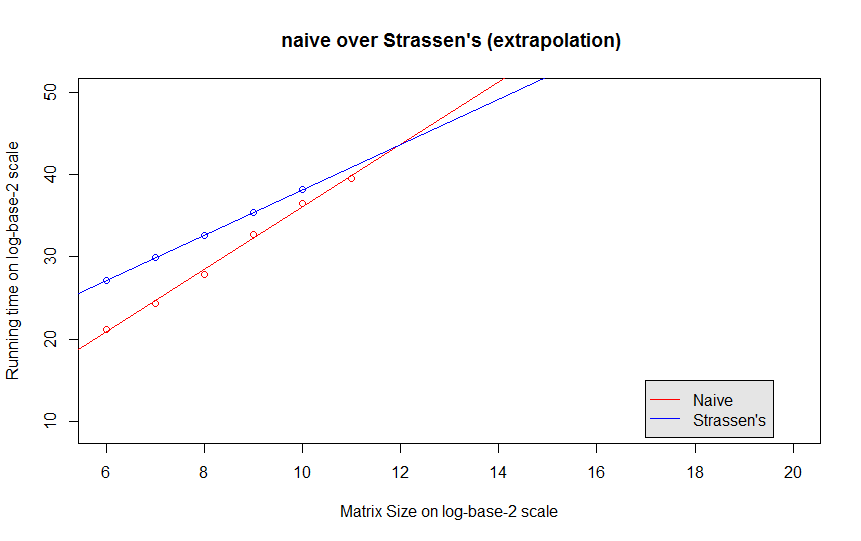
\includegraphics[scale=.35]{graph.png}
  		\caption{We found our results surprising.}
\end{figure}

\subsection{}
Although our intention was to implement Strassen's in parallel, challenges made us
change our plan.

\subsection{}
Our expectations were that with few processors and smaller matrices, the naive algorithm 
would be faster than Strassen’s. As the size of the matrices increased, say beyond 50, or 
number of processors increased, however, our expectation was that Strassen’s would become 
faster than the naive algorithm. What we in fact found was that our machines lacked the 
resources to see Strassen’s overtake the naive algorithm. We simply lacked the time and 
processing power to continue to the point at which Strassen’s would become the faster 
choice. Theoretically, with a large dataset and many processors, Strassen’s is the faster 
option. However, in our application of the algorithms we never made it to the point where 
Strassen’s was faster. So in this case we may have to say that the naive algorithm is 
the ‘better’ option.



\end{document}
